\documentclass{beamer}
\usetheme{Warsaw}

\usepackage[utf8]{inputenc}
\usepackage{fancybox}
\usepackage{multimedia} 
\usepackage{subfig}
\usepackage{amsmath}
\usepackage{hyperref}
\usepackage[all]{xy}
\usepackage{algorithm}
%\usepackage{arevmath}     % For math symbols
\usepackage[noend]{algpseudocode}

\begin{document}



\title[Stochastik] % (optional, only for long titles)
{Stochastik für Informatiker
\\
\includegraphics[scale=0.5]{img/craps}
}
\subtitle{}
\author[Dr. Johannes Riesterer] % (optional, for multiple authors)
{Dr.  rer. nat. Johannes Riesterer}

\date[KPT 2004] % (optional)
{}

\subject{Stochastik}


\begin{frame}
    \frametitle{Stochastik}
\framesubtitle{Inegrierbare Funktionen}
    \begin{block}{Maßraum}
     Ein Meßraum $(\Omega, \mathcal{A})$ ist ein Tupel bestehend aus der Grundmenge $\Omega$ und einer $\sigma$-Algebra $\mathcal{A} \subset  \mathcal{P}(\Omega)$ 
\end{block}

\begin{block}{Maß}
    Ein Maß auf einem Meßraum $(\Omega, \mathcal{A})$ ist Abbildung
    $\mu : \mathcal{A} \to \mathbb{R}_{\geq 0}$
    \begin{align*}
    \mu \biggl(  \bigcup_i A_i  \biggr) = \sum_i \mu(A_i), \text{ mit } A_i \cap A_j = \emptyset \text{ für } i \neq j
    \end{align*}
    \end{block}
    
    \begin{block}{Wahrscheinlichkeitsmaß}
     Ein Maß mit $\mu (\Omega) = 1$ ist ein Wahrscheinlichkeitsmaß.
   \end{block}

 \end{frame}


 \begin{frame}
    \frametitle{Stochastik}
\framesubtitle{Inegrierbare Funktionen}
    \begin{block}{Meßbare Abbildung}
     Eine Abbildung $f:\Omega \to \Omega'$ zwischen zwei Maßräumen 
      $(\Omega, \mathcal{A})$ und $(\Omega', \mathcal{A}')$ heißt meßbar, falls
    \begin{align*}
        f^{-1}(A') \in \mathcal{A} \; \text{für alle } A' \in \mathcal{A}'
    \end{align*}
    \end{block}

    \begin{block}{Meßbare Abbildung}
    Das Urbild jedes Ereignisses ist ein Ereignis
    \end{block}

    \begin{block}{Beispiel}
        Bei endlichen Mengen und Potenzmenge als Sigma-Algebra ist jede Funktion Meßbar.
        Jede stetige Funktion ist meßbar bezüglich Borellscher Sigma-Algebra.
    \end{block}

    
 \end{frame}

 \begin{frame}
    \frametitle{Stochastik}
\framesubtitle{Inegrierbare Funktionen}
    \begin{block}{Konvention}
        Ab jetzt steht $\mathbb{R}^n$ immer für den Maßraum
        $(\mathbb{R}^n, \mathcal{B}(\mathbb{R}^n), \mu)$, wobei $\mathcal{B}(\mathbb{R}^n)$ die Borellsche Sigma-Algebra 
        und $\mu$ das Lebesgue Maß  ist.
    \end{block}

    \begin{block}{Eindeutigkeit}
        Später wichtig: Das Lebesgue Maß ist durch seine Eigenschaften eindeutig bestimmt.
    \end{block}


\end{frame}

\begin{frame}
    \frametitle{Stochastik}
\framesubtitle{}
    \begin{block}{}
        Die Menge der meßbaren Funktionen $f: \Omega \to \mathbb{R}$ bezeichnen wir mit $\mathcal{M}$. 
        Mit $\mathcal{M}^+$ bezeichnen wir die meßbaren Funktionen $f: \Omega \to \mathbb{R}$ mit $f(\omega) \geq 0$. 
    \end{block}

\end{frame}





\begin{frame}
    \frametitle{Stochastik}
\framesubtitle{}
    \begin{block}{Treppenfunktion}
        Eine meßbare Funktion $u: \Omega \to \mathbb{R}$ 
        heißt Treppenfunktion, 
        falls sie nur endlich viele verschiedene Werte annimmt.
    \end{block}


\begin{figure}[H]
    \centering
  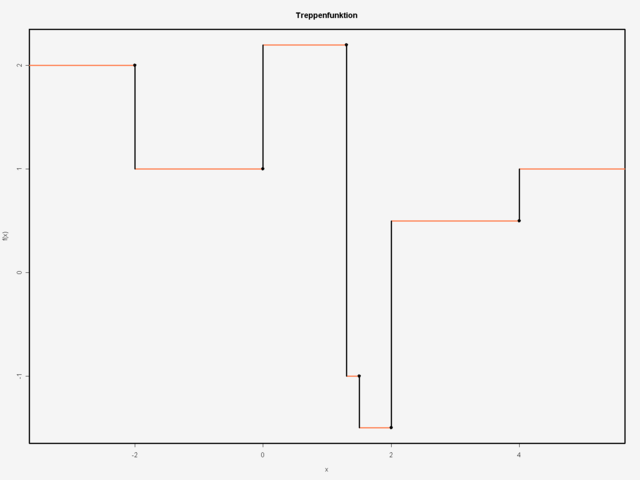
\includegraphics[width=0.6\textwidth]{img/640px-Stepfunction1}
    \caption{Quelle: Wikipedia: https://commons.wikimedia.org/wiki/File:Stepfunction1.png}

\end{figure}
\end{frame}


\begin{frame}
    \frametitle{Stochastik}
\framesubtitle{}
\begin{block}{Indikatorfunktion}
    Für eine Teilmenge $A \subset \mathbb{R}^n$ heißt
    $$ 1_A (x): = \begin{cases} 1 \text{  falls }   x \in A  \\  0  \text{  sonst}  \end{cases}$$
    Indikatorfunktion.
    \end{block}
    
    \begin{figure}[H]
          \centering
        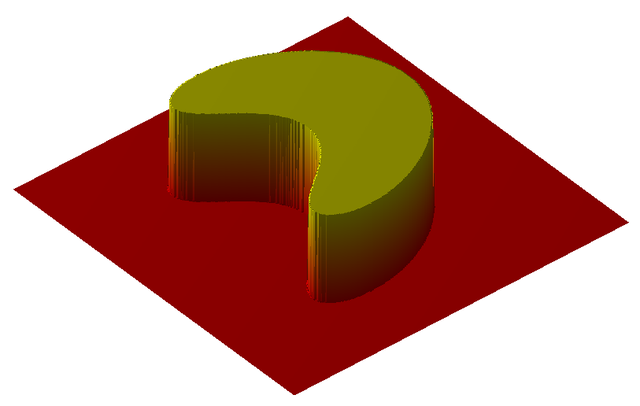
\includegraphics[width=0.5\textwidth]{img/640px-Indicator_function_illustration}
          \caption{Quelle: Wikipedia: https://commons.wikimedia.org/wiki/File:Indicator\_function\_illustration.png}
    
    \end{figure}
\end{frame}


\begin{frame}
    \frametitle{Stochastik}
\framesubtitle{}
    \begin{block}{Darstellung von Treppenfuntkion}
        Eine Treppenfunktion hat eine Darstellung $u = \sum_{i= 1}^n a_i \cdot  1_{A_i}$ mit $A_i \cap A_j = \emptyset$ für $i \neq j$.
    \end{block}

    \begin{block}{Treppenfuntkion}
        Die Menge der Treppenfunktionen bezweichnen wir mit $\mathcal{T}$ und die Treppenfunktionen mit $a_i > 0$ mit $\mathcal{T}^+$.        
    \end{block}
    
    \begin{block}{Eindeutigkeit der Darstellung}
        Sind $u = \sum_{i= 1}^n a_i 1_{A_i} = \sum_{j= 1}^m b_j 1_{B_j}$ zwei verschiedene Darstellungen einer Treppenfunktion 
        $u \in \mathcal{T}^+$
        so ist $\sum_{i= 1}^n a_i \mu (A_i) = \sum_{j= 1}^m b_j \mu (B_j)$
    \end{block}




\end{frame}


\begin{frame}
    \frametitle{Stochastik}
\framesubtitle{}
    \begin{block}{Integral einer Treppenfunktion}
        Für eine Treppenfunktion $u \in \mathcal{T}^+$ definieren wir
\begin{align*}
    \int_\Omega u \; d\mu= \sum_{i=1}^n a_i \mu(A_i)
\end{align*}
Diese ist unabhängig von der Darstellung.
    \end{block}

\end{frame}


\begin{frame}
    \frametitle{Stochastik}
\framesubtitle{}
\begin{block}{Eigenschaften des Integrals von Treppenfunktionen}
    Sind $u$ und $v$ zwei Treppenfunktionen, dann gilt:
    \begin{itemize}
    \item $\int_{\Omega} 1_A  d\mu  = \mu (A)$  
    \item $\int_{\Omega} \alpha u  + \beta v d\mu = \alpha \int_{\Omega}  u d\mu + \beta  \int_{\Omega}  v d\mu$
    \item Ist $u(x) \leq v(x)$ für alle $x$, so ist $\int_{\Omega} u d\mu \leq \int_{\Omega} v d\mu$ 
    \end{itemize}
    \end{block}
\end{frame}


\begin{frame}
    \frametitle{Stochastik}
\framesubtitle{}
    \begin{block}{Meßbare Abbildungen}
        Eine nicht negative Funktion $f:\Omega \to \mathbb{R}$ ist genau dann meßbar, wenn
        es eine Folge $u_n \in \mathcal{T}^+$ gibt mit $u_n \uparrow f$.
    \end{block}

\end{frame}


\begin{frame}
    \frametitle{Stochastik}
\framesubtitle{}
Sei $u_n \in \mathcal{T}^+$: \\
Müssen zeigen, dass Grenzwert auch in $\mathcal{T}^+$ liegt.
Dies liegt im Wesentlichen daran, dass der Limes ein inf-sup ist und dieser Vereinigung von meßbaren Mengen ist.
\\
Sei nun umgekehrt $f \in \mathcal{M}^+$ meßbar: \\
definiere
\begin{align*}
    A_{j,n} : = \begin{cases} 
        \{ \frac{j}{2^n} \leq f \leq \frac{j+1}{2^n} \} \text{ für } j= 0, \dots, n \cdot 2^n -1 \\
        \{  f \geq n \} \text{ für } j= n \cdot 2^n 
    \end{cases}
\end{align*}
und damit 
\begin{align*}
    u_n : =  \sum_{j= 0}^{n2^n} \frac{j}{2^n} 1_{A_{j,n}}
\end{align*}
Damit gilt $u_n(x) \leq f(x) \leq u_n(x) +2^{-n}$.
\end{frame}



 
\begin{frame}
    \frametitle{Stochastik}
\framesubtitle{}
    \begin{block}{Integral nicht negativer meßbarer Funktionen}
        Für eine Funktion $f \in \mathcal{M}^+$ definieren wir
        \begin{align*}
            \int_{\Omega} f \;  d \mu := \lim_{n \to \infty} \int_{\Omega} u_n \; d \mu  
        \end{align*}
        wobei $u_n \in \mathcal{T}^+$ eine Folge von Treppenfunktionen ist mit 
        $u_n \uparrow f$.

        
    \end{block}
    \begin{block}{!!}
    Müssen zeigen, dass diese Definition unabhängig ist von der Folge der Treppenfunktionen.
\end{block}
\end{frame}




\begin{frame}
    \frametitle{Stochastik}
\framesubtitle{}
    \begin{block}{}
        Für jede wachsende Folge $(u_n) \in \mathcal{T}^+$ und jedes $v \in \mathcal{T}^+$ mit $v \leq \lim_{n \to \infty} u_n$ gilt
        \begin{align*}
            \int_{\Omega} v \;  d \mu \leq \lim_{n \to \infty} \int_{\Omega} u_n \; d \mu  
        \end{align*}
    \end{block}

\end{frame}


\begin{frame}
    \frametitle{Stochastik}
    Sei $v = \sum_{i=1}^{m} a_i 1_{A_i}$.  
    Für festes $\beta > 1$ setze $B_n: = \{\beta u_n \geq v \}$.
    Damit gilt $B_n \uparrow \Omega$ und $\beta u_n \geq v \cdot 1_{B_n}$ und man erhält
    \begin{align*}
        \int_{\Omega} v \;  d \mu & = \sum_{i=1}^n a_i \mu (A_i) = \lim_{n \to \infty} \sum_{i=1}^n a_i \mu (A_i \cap B_n) \\
        & = \lim_{n \to \infty} \int_{\Omega} v \cdot 1_{B_n}\;  d \mu
        \leq \lim_{n \to \infty} \beta \int_{\Omega} u_n \;  d \mu = \beta \lim_{n \to \infty} \int_{\Omega} u_n \;  d \mu
    \end{align*}
    Mit $\beta \to 1$ folgt die Behauptung.
\framesubtitle{}
\end{frame}


\begin{frame}
    \frametitle{Stochastik}
\framesubtitle{}
         Sind nun $u_n, v_n \in \mathcal{T}^+$ zwei wachsende Folgen mit
          $\lim_{n \to \infty} u_n = \lim_{n \to \infty} v_n$ so gilt
          $\int_{\Omega} v_k \; d \mu \leq \lim_{n \to \infty} \int_{\Omega} v_k \; d \mu$ und damit 
          $\lim_{k \to \infty} \int_{\Omega} v_k \; d \mu  \leq \lim_{n \to \infty} \int_{\Omega} v_k \; d \mu$. 
          Aus Symmetriegründen folgt die Unabhängigkeit der Definition von der Wahl der Folgen von Treppenfunktionen.
\end{frame}



\begin{frame}
    \frametitle{Stochastik}
\framesubtitle{}
    \begin{block}{Integral für meßbare Funktionen}
        Für eine meßbare Funktion  $f \in \mathcal{M}$ setzen wir
        $$ \int_{\Omega} f \; d\mu = \int_{\Omega}f^+ \; d\mu  - \int_{\Omega}-f^- \; d\mu$$
        wobei $f^+(x) := \max (0, f(x))$ und $f^-(x) := \min (0, f(x))$
    \end{block}

    \begin{block}{Integral für meßbare Funktionen}
       Eine meßbare Funktion heißt integrierbar, falls ihr Integral endlich ist.
    \end{block}

\end{frame}

\begin{frame}
    \frametitle{Stochastik}
\framesubtitle{}
\begin{block}{Eigenschaften des Integrals}
    Sind $f$ und $g$ zwei meßbare Funktionen, dann gilt:
    \begin{itemize}
        \item $\int_{\Omega} 1_A  d\mu  = \mu (A)$  
    \item $\int_{\Omega} \alpha f  + \beta g d\mu = \alpha \int_{\Omega}  f d\mu + \beta  \int_{\Omega}  g d\mu$
    \item Ist $f(x) \leq g(x)$ für alle $x$, so ist $\int_{\Omega} f d\mu \leq \int_{\Omega} g d\mu$ 
    \item $ \biggl | \int_{\Omega} f \; d\mu \biggr | \leq \int_{\Omega} |f| \; d\mu $
    \end{itemize}
    \end{block}
\end{frame}

\begin{frame}
    \frametitle{Angewandte Mathematik}
\framesubtitle{Fubini}
\begin{figure}[H]
      \centering
    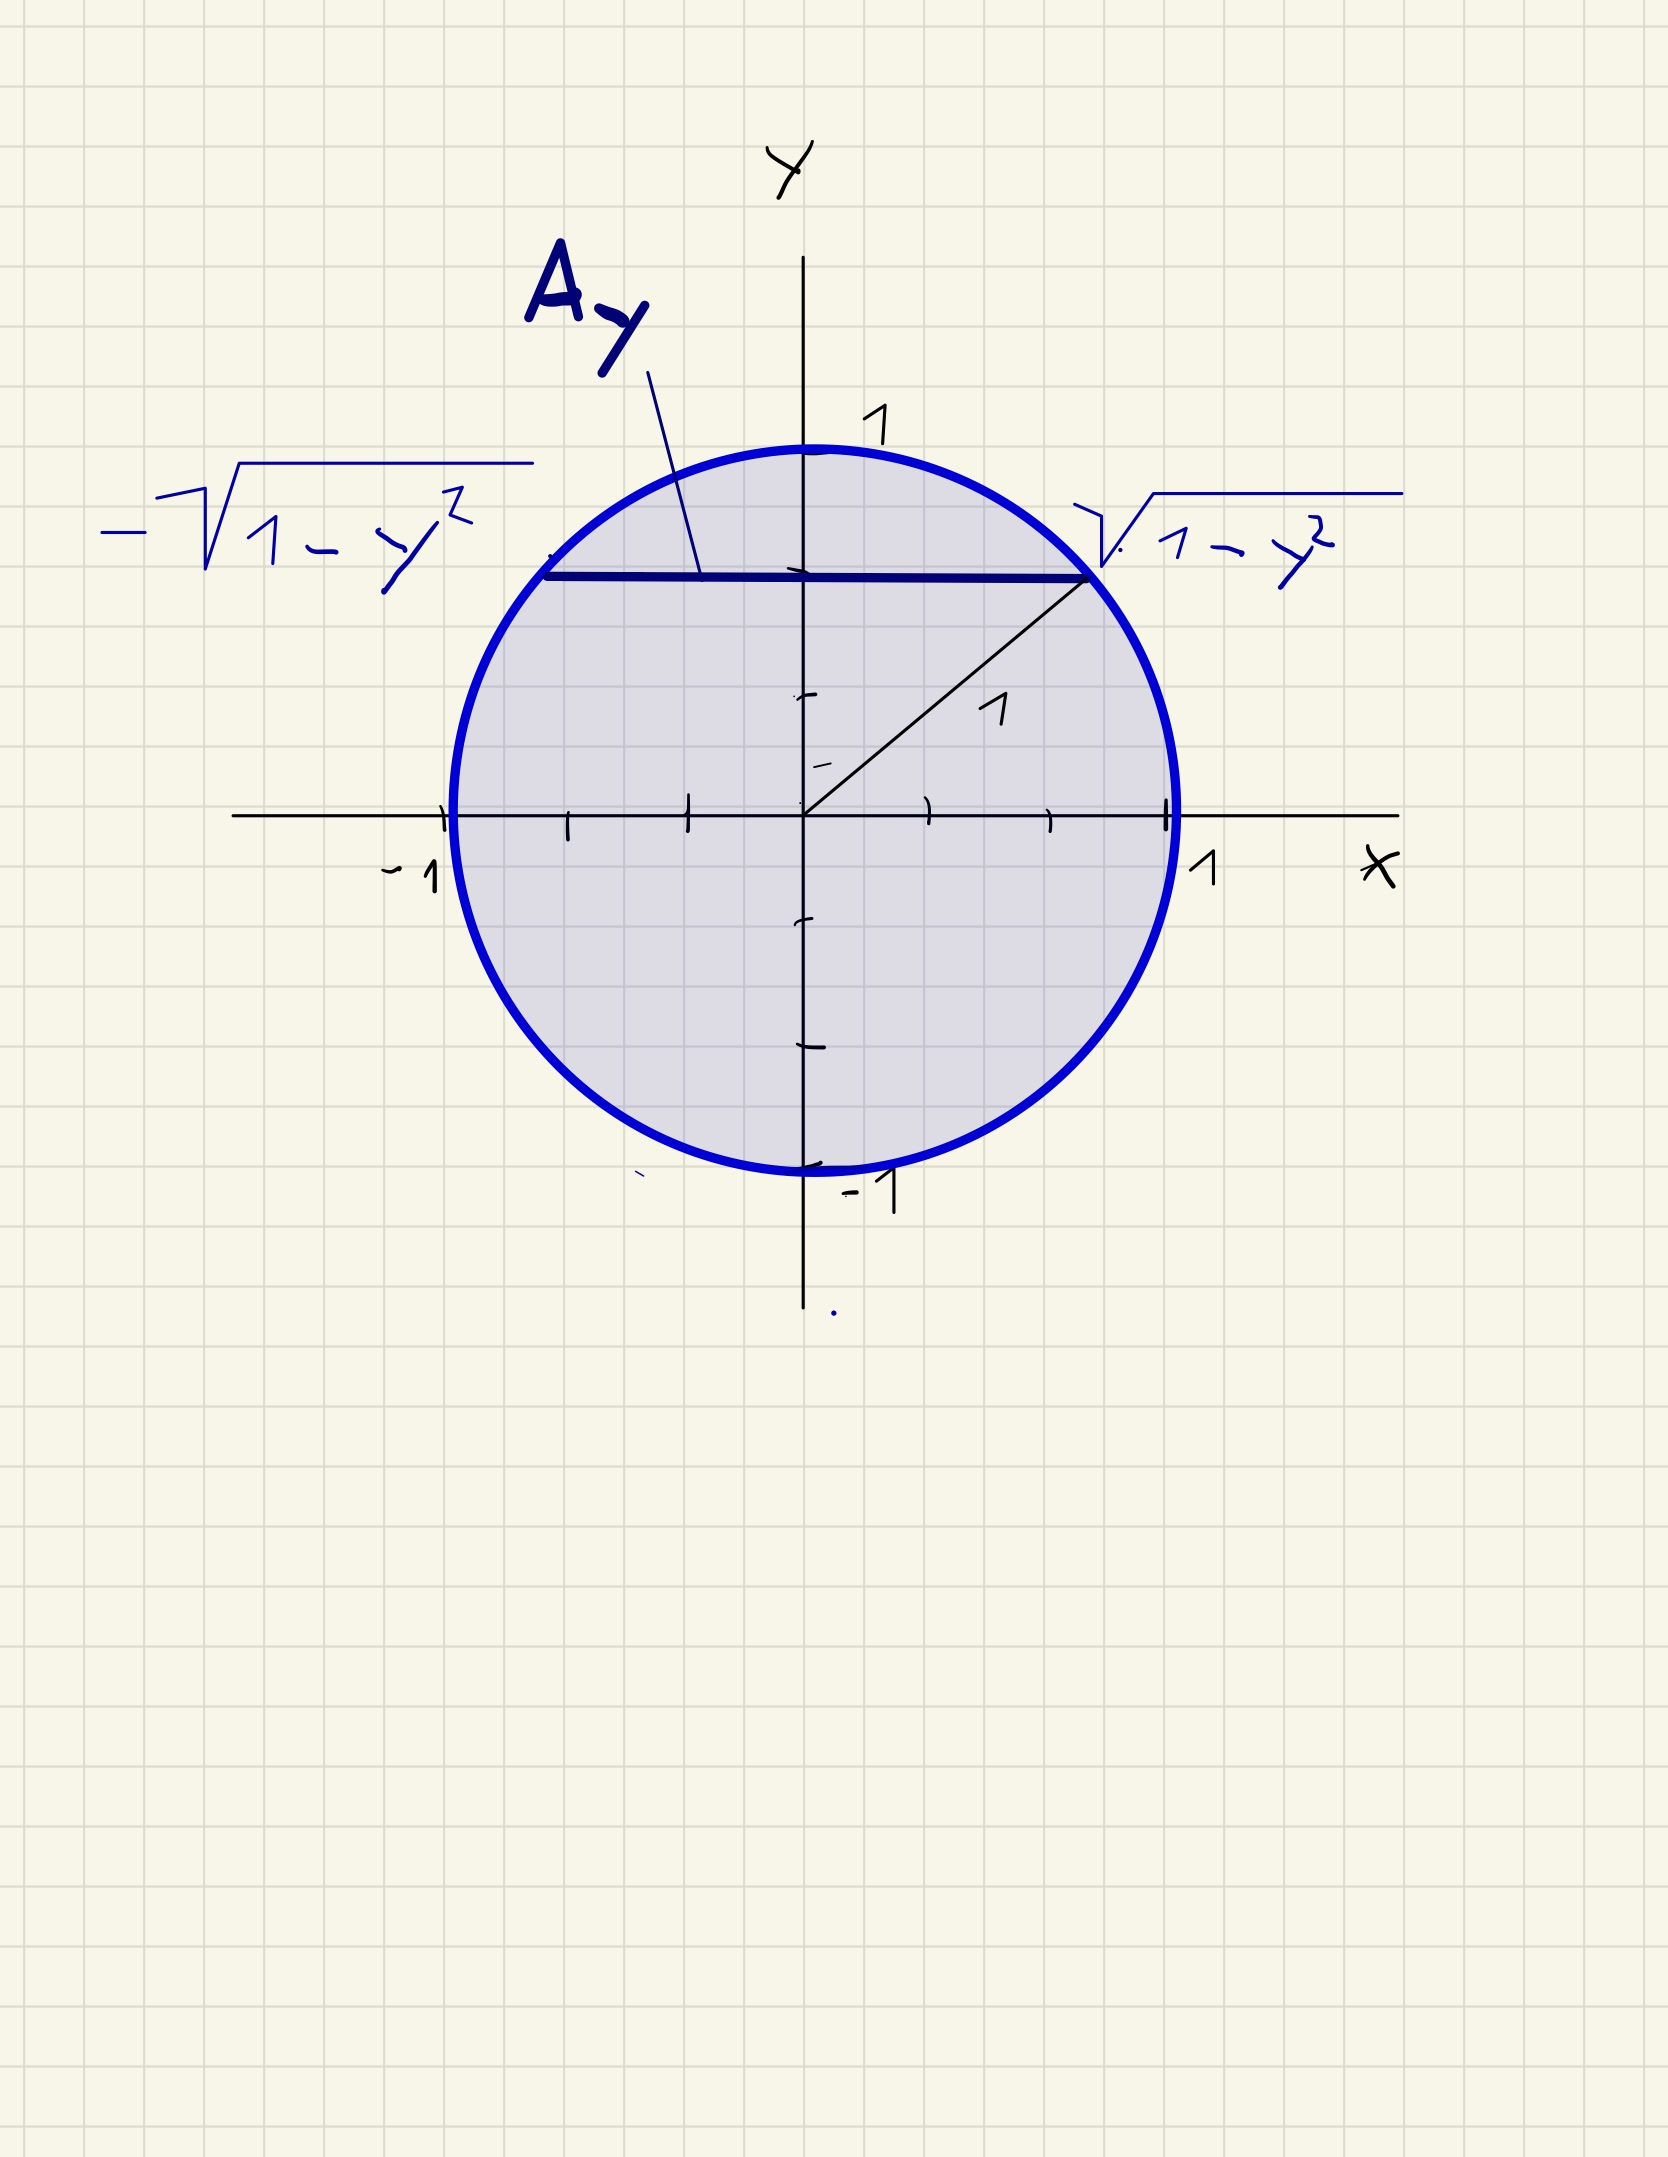
\includegraphics[width=0.8\textwidth]{img/Kreis}
\end{figure}
 \end{frame}

 \begin{frame}
    \frametitle{Angewandte Mathematik}
    \framesubtitle{Fubini}
    \begin{block}{Beispiel}
Sei $K := B^2_1(0) := \{   (x,y) \in \mathbb{R}^2 \; | \; \sqrt{x^2 + y^2 } \leq 1\}$. Anschaulich ist
\begin{align*}
\mu_2(K) &  = \int_{\mathbb{R}^2} 1_K  d \mu =  \int_{-1}^{1} \biggl ( \int_{-\sqrt{1- y^2}}^{\sqrt{1- y^2}} 1 dx \biggr ) dy = \\ 
& =  2 \int_{-1}^{1}  \sqrt{1 - y^2}   \; dy  \\ 
 & (substitution \;   y = sin(u)) =   2 \int_{-\frac{\pi}{2}}^{\frac{\pi}{2}}   \cos(u)^2   \; du = 2 \cdot \frac{\pi}{2} = \pi
\end{align*}
\end{block}
 \end{frame}
 
 \begin{frame}
    \frametitle{Stochastik}
\framesubtitle{Fubini}
    \begin{block}{Fubini}
        Für eine integrierbare Funktion $f: \mathbb{R}^n \to \mathbb{R}$ gilt
        \begin{align*}
        \int_{\mathbb{R}^{n-k} \times \mathbb{R}^{k}} f \; d\mu_n  =  \int_{\mathbb{R}^{n-k}}  \int_{\mathbb{R}^k}  f \; d\mu_{n-k} \;  d\mu_k  
        \end{align*}
    \end{block}

\end{frame}

\begin{frame}
    \frametitle{Stochastik}
\framesubtitle{Fubini}
Beweisidee:

\begin{block}{Schnittmenge}
Sei $ A \subset \mathbb{R}^n$. Für $ y \in \mathbb{R}^k$ heißt
$$ A_y :=  \biggl \{    x \in \mathbb{R}^{n-k}  \; | \;  (x,y) \in A \biggr \}$$  
Schnittmenge von $A$ zu $y$.
\end{block}

\begin{block}{Schnittmenge}
    Für $A \subset \mathbb{R}^n $ erhält man ein Maß
    $$ \mu'(A) := \int_{\mathbb{R}^k} \mu_{n-k}(A_y) d \mu_k$$ 
\end{block}
Aufgrund der Eindeutigkeit des Lebesgue Maßes folgt die Behauptung.
\end{frame}


\end{document}

